\documentclass[11pt,a4paper,twoside]{book}
\usepackage[utf8]{inputenc}
\usepackage[spanish]{babel}
\usepackage{amsmath}
\usepackage{graphicx}
\usepackage{amsfonts}
\usepackage{amssymb}
\usepackage[left=2cm,right=2cm,top=2cm,bottom=2cm]{geometry}
\usepackage{float}
\author{Víctor de Tejada Molera}
\begin{document}
\chapter{Resultados de los experimentos}
    En este apartado se muestran los resultados obtenidos de los diferentes test perceptuales que se han realizado a lo largo del proyecto. 
    \section{Resultados del test previo}
        Como ya se comentó en apartados anteriores, en este test previo el objetivo consiste en comprobar que los participantes podían realmente distinguir los estímulos cuando se correspondían a las de las posiciones más alejadas entre sí. También se quiere comprobar que la sala es lo suficientemente simétrica como para simplificar la toma de datos a una de las mitades del auditorio. De esta forma se han obtenido 70 preguntas que pueden agruparse en cuatro casos posibles: 
        \begin{itemize}
            \item \textbf{Butacas separadas horizontalmente}: Los audios se corresponden a posiciones en la misma fila, pero distinta butaca.
            \item \textbf{Butacas separadas verticalmente}: Las señales se corresponden con posiciones en distinta fila, pero mismo número de butaca.
            \item \textbf{Butacas separadas tanto vertical como horizontalmente}: Los audios se corresponden a posiciones diferentes tanto de fila como de butaca.
            \item \textbf{butacas en la misma posición}: La fila y el número de butaca para las dos señales es la misma.
        \end{itemize}
        Este test, como ya se comentó anteriormente, fue realizado por un total de 10 personas, con 7 preguntas por persona. Los resultados totales pueden observarse en la tabla \ref{tablaTestPrevio}. Para cada caso, se ha desglosado el número total de respuestas para cada posible distribución de posiciones, el número de respuestas marcadas como diferentes e iguales (independientemente del nivel de seguridad), y el número de respuestas marcadas con un ``Nivel de seguridad: poca'' en función de la respuesta. En el anexo F se encuentra una tabla con cada uno de los resultados individuales con el nombre de cada posición exacta.
        
        \begin{table}[H]
			\begin{center}
			\begin{scriptsize}
			\begin{tabular}{| c | c | c | c | c | c |}
			    \hline
				\textbf{Separación butacas}&\textbf{Respuestas}&\textbf{Iguales}&\textbf{Diferentes}&\textbf{Duda iguales}&\textbf{Duda diferentes}\\ \hline
                Horizontal&27&9&18&2&2\\ \hline
                Vertical&10&1&9&0&1\\ \hline
                Horizontal y vertical&23&5&18&1&2\\ \hline
                Misma posición&10&9&1&1&0\\ \hline
			\end{tabular}
			\caption{Resultados del test previo.}
			\label{tablaTestPrevio}
			\end{scriptsize}
			\end{center}	
		\end{table}	
	\section{Resultados del test final}
	    Para este test, se han agrupado los resultados de dos formas de manera que resulta más fácil entenderlos para el análisis que se realiza más adelante en el apartado de ``Análisis estadístico''. La primera forma de organización es en función de la distancia relativa entre butacas.Para este tipo de agrupación, los resultados son los mostrados en la tabla \ref{tablaTestButacas} que muestran los resultados de las 34 personas que participaron en el test produciendo un total de 850 respuestas. Esta separación se indica en la primera columna con intervalos de la forma $[x-y)$ donde se expresa el rango de distancias en las que se incluyen las respuestas. Por ejemplo, el intervalo $[2-3)$ incluye todas las respuestas en las que la distancia relativa entre butacas se encuentra entre los 2 metros (incluidos) y los 3 metros (sin incluir). 
	    
	    \begin{table}[H]
			\begin{center}
			\begin{scriptsize}
			\begin{tabular}{| c | c | c | c | c | c |}
			    \hline
				\textbf{Distancia [m]}&\textbf{Respuestas}&\textbf{Iguales}&\textbf{Diferentes}&\textbf{Duda iguales}&\textbf{Duda diferentes}\\ \hline
                (0-2)&61&40&21&11&9\\ \hline
                [2-3)&76&40&36&11&16\\ \hline
                [3-4)&102&47&55&14&14\\ \hline
                [4-5)&111&30&81&13&29\\ \hline
                [5-6)&95&24&71&9&21\\ \hline
                [6-7)&78&11&67&6&10\\ \hline
                [7-8)&70&9&61&2&4\\ \hline
                [8-9)&52&4&48&3&9\\ \hline
                [9-10)&62&3&59&1&8\\ \hline
                [10-11)&47&1&46&0&3\\ \hline
                [11-12)&33&1&32&0&2\\ \hline
                [12-14)&33&1&32&1&0\\ \hline
                [14-18)&24&0&24&0&1\\ \hline \hline
                \textbf{Total}&844&211&633&71&126\\ \hline
			\end{tabular}
			\caption{Resultados del test final en función de la distancia entre butacas.}
			\label{tablaTestButacas}
			\end{scriptsize}
			\end{center}	
		\end{table}
		
		La otra forma de organización de los datos es ordenandolos en función de la distancia relativa a la fuente sonora (considerando esta como un origen de coordenadas). En este caso, la agrupación sigue la misma nomenclatura que en el caso anterior, sólo que esta vez el intervalo $[x-y)$ se corresponde con las distancias promedio a cada pareja a la fuente, en vez de la distancia entre butacas. Haciendo esta organización, los datos se reparten de la forma que se muestra en la tabla \ref{tablaTestFuente}
		
		\begin{table}[H]
			\begin{center}
			\begin{scriptsize}
			\begin{tabular}{| c | c | c | c | c | c |}
			    \hline
				\textbf{Distancia [m]}&\textbf{Respuestas}&\textbf{Iguales}&\textbf{Diferentes}&\textbf{Duda iguales}&\textbf{Duda diferentes}\\ \hline
                [6-8)&15&5&10&2&2\\ \hline
                [8-10)&35&10&25&2&3\\ \hline
                [10-11)&32&8&24&2&7\\ \hline
                [11-12)&53&12&41&7&7\\ \hline
                [12-13)&55&14&41&3&5\\ \hline
                [13-14)&67&14&53&6&9\\ \hline
                [14-15)&101&22&79&10&10\\ \hline
                [15-16)&99&18&81&3&12\\ \hline
                [16-17)&84&18&66&4&12\\ \hline
                [17-18)&63&10&53&3&11\\ \hline
                [18-19)&95&21&74&3&15\\ \hline
                [19-20)&62&19&43&11&9\\ \hline
                [20-21)&44&19&25&9&10\\ \hline
                [21-24]&39&21&18&6&4\\ \hline \hline
                \textbf{Total}&844&211&633&71&126\\ \hline
			\end{tabular}
			\caption{Resultados del test final en función de la distancia relativa a la fuente.}
			\label{tablaTestFuente}
			\end{scriptsize}
			\end{center}	
		\end{table}
		
		Para el cálculo de ambas distancias, se ha generado un script en Python que extrae la información de la posición de recepción de cada fichero de audio que se encuentra en el nombre de dicho archivo y las distancias medidas presencialmente en el auditorio (toda esta información se comentó en el apartado de ``Toma de datos'').
		
		Tomando esta información se hace el cálculo de las distancias para todos los casos que se han producido durante la realización de los test y que han quedado recogidas en el fichero csv. En la figura \ref{fig:calcDist} se puede observar un ejemplo gráfico sobre cómo se han calculado dichas distancias y en el anexo C se puede consultar el código de Python en su totalidad.
		
		\begin{figure}[H]
                \begin{center}
                    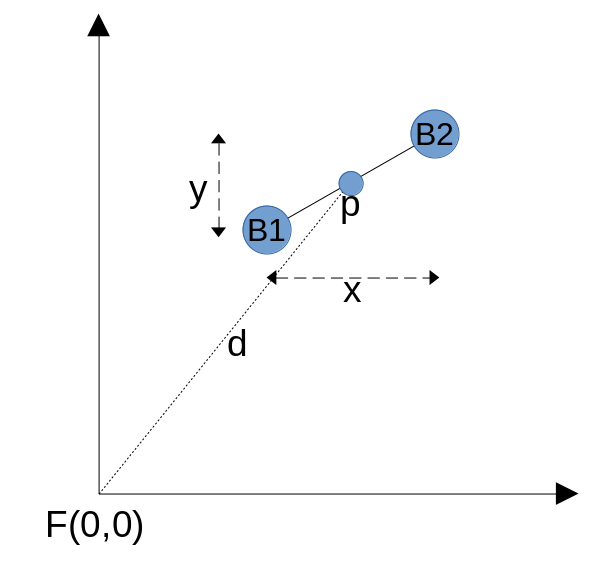
\includegraphics[scale=.4]{../imagenes/calculoDistancia.png}
                    \caption{Ejemplo gráfico del cálculo de la distancia a la fuente.}
                    \label{fig:calcDist}
                \end{center}
            \end{figure}
		
		Para ambas distribuciones se han eliminado los resultados en los que la posición de las butacas es la misma ya que el análisis es diferente para la similitud que para la diferencia y, como se mostrará en el apartado de ``Análisis del test previo'', los participantes detectaron sin problemas cuando ambas señales son exactamente idénticas. Por este motivo, ya no se consideró necesario incluirlas.

\end{document}